
\subsection{Search Termination}\label{subsubsec:SeachTerminationMethodology}
\workinprogress

At each discrete timestep, the agent can either choose to move to a new grid location to record a sensor measurement or it can decide to terminate the search based on its estimated state of the environment. There is a trade-off in terminating the search early, which means that less time and resources are spent on continuing the search, versus the possibility of drawing misinformed conclusions from the search due to a lack of information. For example, if the agent receives a series of false positive readings at a given location, it could mistakenly choose to conclude that the target is present at a given location rather than sample further to gain confidence that it has correctly found the location of the target. Following this line of thinking, it is clear that a strategy needs to be devised to minimize the probability of drawing false conclusions, which is described in the performance measure set out in \ref{sssection:PerfMeas}.\par
Previous related work, \cite{Chung2007ASearchb} has addressed this problem using methods that use heuristics as well as a more formal asymptotic theory-based approach. We ultimately choose to implement the Sequential Probability Ratio Test (SPRT), which is a hypothesis-testing framework developed by \citeauthor{Wald1950BayesProblems} to optimally deal with sequential decision problems, as opposed to traditional frameworks which assume that all the necessary data has been gathered prior to analysis \cite{Wald1950BayesProblems}. The background knowledge behind the SPRT can be found in section \ref{subsec:SPRT}. An algorithm is also provided on how to perform this test in practice.
%The details of the proof of optimality of the SPRT is given in \cite{Wald1950BayesProblems} and we have outlined the details of how to perform hypothesis-testing using this framework in section <refer to the section>, along with the practical advantages and drawbacks of using it. 
We applied the SPRT algorithm to our problem to provide a search termination criteria using the following quantities: 
%In order to allow the agent to make a decision on whether to terminate the search or not, the following procedure was used: \note{Might be worthwhile simply outlining the algorithm}

\begin{gather}\label{eqn:SearchStatus}
H_0 : \text{The null hypothesis, the target is not present in the search region}\nonumber
\\ \nonumber
H_1 : \text{The alternative hypothesis, the target is present in the search region}\nonumber
\\ \nonumber
\alpha : \text{The maximum probability of making a type } \Romannum{1} \text{ error.} \nonumber
\\ \nonumber
\beta : \text{The maximum probability of making a type } \Romannum{2} \text{ error.}\nonumber
\\ \nonumber
\\ \nonumber
p_{0t} : \text{ The probability of observing the data $(e_1, ..., e_t)$ under the assumption of $H_0$ =} \nonumber
\\ \nonumber
\sum_{loc=1}^{n} p(TargetLoc_t = loc, AgentLoc_t, SearchStatus_t| e_{1:t}, u_{1:t})\nonumber
\\ \nonumber
\\ \nonumber
p_{1t} : \text{ The likelihood of observing the data $(e_1, ..., e_t)$ under the assumption of $H_1$ =} \nonumber
\\ \nonumber
p(TargetLoc_t = n+1, AgentLoc_t, SearchStatus_t | e_{1:t}, u_{1:t})\nonumber 
\end{gather}

$p_{0t}$ and $p_{1t}$ are calculated by using the evidence likelihood algorithm, which is described in detail in section \ref{subsubsec:EvLikelihood}. The SPRT algorithm was then used at each timestep to decide whether to 
\begin{enumerate}
    \item Terminate the search accepting $H_0$, that the target is not present in the search region.
    \item Terminate the search accepting $H_1$, that the target is present in the search region. In this case, the target location with the highest estimated probability is returned as the target location.
    \item Continue the search, using the Action Selection Strategy described in section \ref{subsubsec:ActionSelection}.
\end{enumerate}
In practice, we often took log transforms of the values used in the SPRT, to simplify some calculations and to be able to look at plots that are less skewed and easier to interpret.

\subsection{Analysis of Search Termination Criteria}
The two parameters, $\alpha$ and $\beta$ that the user needs to specify to perform the Sequential Probability Ratio test need to be chosen carefully and depend on the context of the search. As in the usual hypothesis testing context, it is important to consider the significance level and power of the test to ensure that they reflect the severity of drawing an incorrect conclusion. Figure \ref{fig:SPRTVaryingT1} shows how the varying the type \Romannum{1} error rate for a fixed type \Romannum{2} error rate affects the upper and lower threshold for cutting off the search. Figure \ref{fig:SPRTVaryingT2} shows how the varying the type \Romannum{2} error rate for a fixed type \Romannum{1} error rate affects the upper and lower threshold for cutting off the search. Note that as the varying error rate increases on the x-axis, the decision boundaries come closer together, reflecting the intuition that we are more willing to accept a mistake.

\note{might be better to have figures side-by-side.}
%\begin{figure}
%    \centering
%    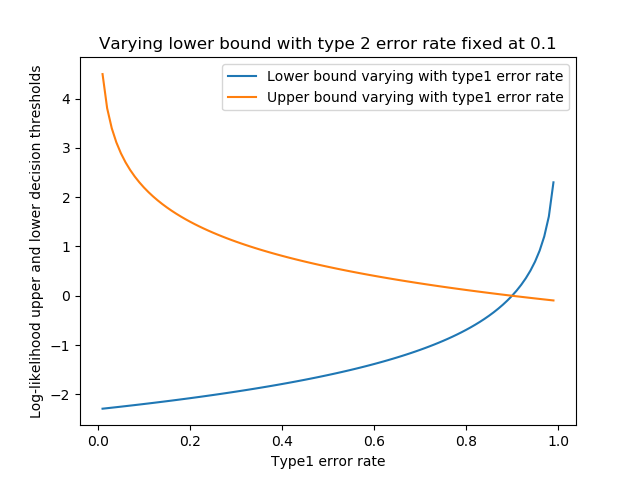
\includegraphics[width = 0.75\linewidth]{Chapters/MultiAgentTargetDetection/Figs/SearchTermination/SPRTDecisionThresholdVaryingT1ErrorRate.png}
%    \caption{The Log-likelihood upper and lower threshold for a varying type \Romannum{1} error rate and fixed type \Romannum{2} error rate.}
%    \label{fig:SPRTVaryingT1}
%\end{figure}

%\begin{figure}
%    \centering
%    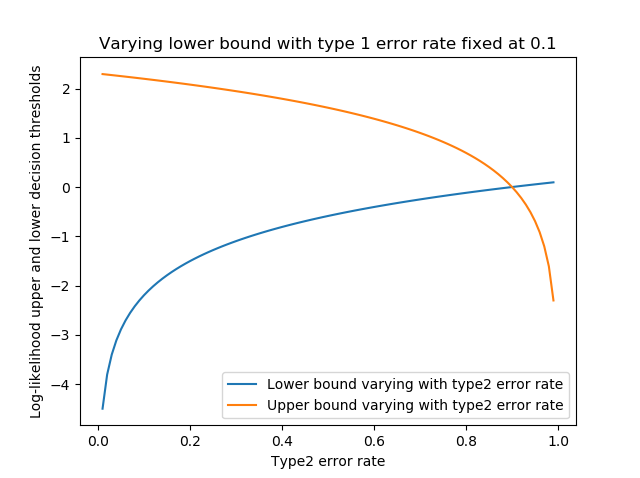
\includegraphics[width = 0.75\linewidth]{Chapters/MultiAgentTargetDetection/Figs/SearchTermination/SPRTDecisionThresholdVaryingT2ErrorRate.png}
%    \caption{The Log-likelihood upper and lower threshold for a varying type \Romannum{2} error rate and fixed type \Romannum{1} error rate.}
%    \label{fig:SPRTVaryingT2}
%\end{figure}


\begin{figure}%
    \centering
    \subfloat[Varying T \Romannum{1} error rate and fixed T \Romannum{2} error rate]{{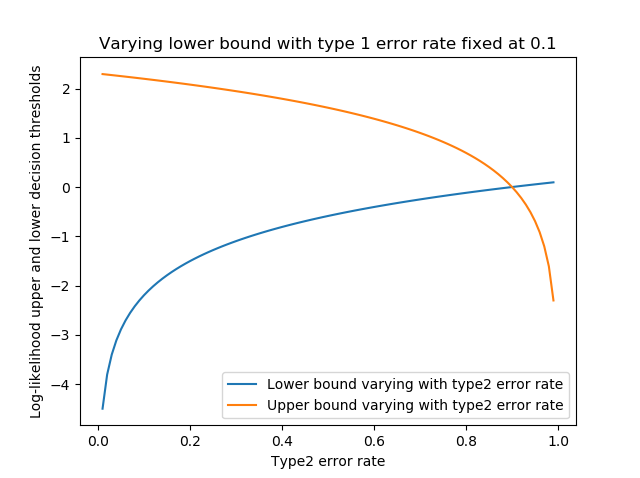
\includegraphics[width=7cm]{Chapters/MultiAgentTargetDetection/Figs/SearchTermination/SPRTDecisionThresholdVaryingT2ErrorRate.png} }}%
    \qquad
    \subfloat[Varying T \Romannum{2} error rate and fixed T \Romannum{1} error rate]{{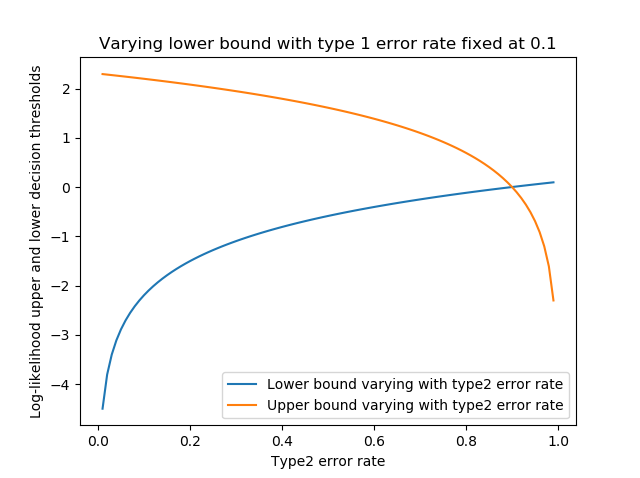
\includegraphics[width=7cm]{Chapters/MultiAgentTargetDetection/Figs/SearchTermination/SPRTDecisionThresholdVaryingT2ErrorRate.png} }}%
    \caption{Upper and lower values of A and B for varying error rates. Values are shown on a log scale}%
    \label{fig:example}%
\end{figure}



\begin{figure}
    \centering
    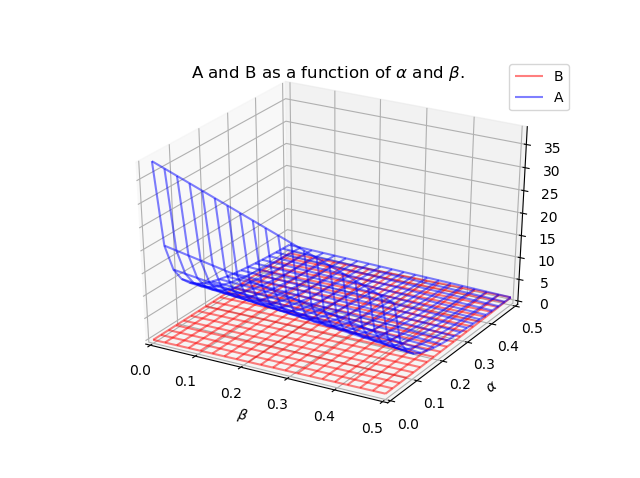
\includegraphics[width = 0.75\linewidth]{Chapters/MultiAgentTargetDetection/Figs/SearchTermination/AandBAsFunctionOfAlphaAndBeta.png}
    \caption{The upper and lower SPRT bounds for acceptance and rejection of $H_0$, as functions of the significance and power of the test. Values are shown on a log scale.}
    \label{fig:SPRTCutoffFunctionOfAlphaAndBeta}
\end{figure}



\begin{figure}
    \centering
    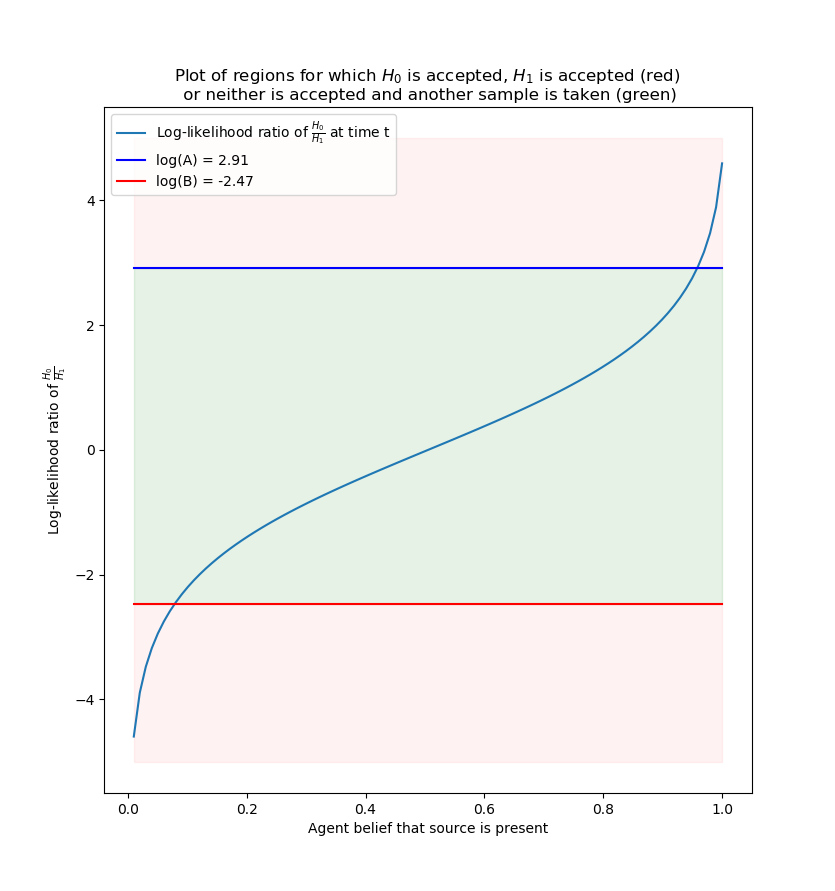
\includegraphics[width = 0.75\linewidth]{Chapters/MultiAgentTargetDetection/Figs/SearchTermination/CutoffRegions.png}
    \caption{The cutoff regions of the SPRT for $\alpha=0.05$, $\beta=0.08$ as a function of agent belief in whether target is present or not. Values are shown on a log scale.}
    \label{fig:SPRTLogLikelihoodRatio}
\end{figure}




\note{maybe move tables to appendix}
\begin{table}[!ht]
\centering
\caption{Upper threshold of SPRT, $A$,  as a function of $\alpha$ and $\beta$}
\begin{tabular}{| c |cccccccccc|} 
\toprule
\diagbox{$\beta$}{$\alpha$} & \makecell{0.05}& \makecell{0.1} & \makecell{0.15} & \makecell{0.2}& \makecell{0.25}& \makecell{0.3} & \makecell{0.35}& \makecell{0.4}& \makecell{0.45}& \makecell{0.5}  \\ 
\midrule
0.05 & 19.00 & 18.00 & 17.00 & 16.00 & 15.00 & 14.00 & 13.00 & 12.00 & 11.00 & 10.00 \\
0.1 & 9.50 & 9.00 & 8.50 & 8.00 & 7.50 & 7.00 & 6.50 & 6.00 & 5.50 & 5.00 \\
0.15 & 6.33 & 6.00 & 5.67 & 5.33 & 5.00 & 4.67 & 4.33 & 4.00 & 3.67 & 3.33 \\
0.2 & 4.75 & 4.50 & 4.25 & 4.00 & 3.75 & 3.50 & 3.25 & 3.00 & 2.75 & 2.50 \\
0.25 & 3.80 & 3.60 & 3.40 & 3.20 & 3.00 & 2.80 & 2.60 & 2.40 & 2.20 & 2.00 \\
0.3 & 3.17 & 3.00 & 2.83 & 2.67 & 2.50 & 2.33 & 2.17 & 2.00 & 1.83 & 1.67 \\
0.35 & 2.71 & 2.57 & 2.43 & 2.29 & 2.14 & 2.00 & 1.86 & 1.71 & 1.57 & 1.43 \\
0.4 & 2.37 & 2.25 & 2.12 & 2.00 & 1.88 & 1.75 & 1.62 & 1.50 & 1.38 & 1.25 \\
0.45 & 2.11 & 2.00 & 1.89 & 1.78 & 1.67 & 1.56 & 1.44 & 1.33 & 1.22 & 1.11 \\
0.5 & 1.90 & 1.80 & 1.70 & 1.60 & 1.50 & 1.40 & 1.30 & 1.20 & 1.10 & 1.00 \\
\bottomrule
\end{tabular}
\end{table}



\begin{table}[!ht]
\centering
\caption{Lower threshold of SPRT, $B$, as a function of $\alpha$ and $\beta$}
\begin{tabular}{| c |cccccccccc|} 
\toprule
\diagbox{$\beta$}{$\alpha$} & \makecell{0.05}& \makecell{0.1} & \makecell{0.15} & \makecell{0.2}& \makecell{0.25}& \makecell{0.3} & \makecell{0.35}& \makecell{0.4}& \makecell{0.45}& \makecell{0.5}  \\ 
\midrule
0.05 & 0.05 & 0.11 & 0.16 & 0.21 & 0.26 & 0.32 & 0.37 & 0.42 & 0.47 & 0.53 \\
0.1 & 0.06 & 0.11 & 0.17 & 0.22 & 0.28 & 0.33 & 0.39 & 0.44 & 0.50 & 0.56 \\
0.15 & 0.06 & 0.12 & 0.18 & 0.24 & 0.29 & 0.35 & 0.41 & 0.47 & 0.53 & 0.59 \\
0.2 & 0.06 & 0.12 & 0.19 & 0.25 & 0.31 & 0.37 & 0.44 & 0.50 & 0.56 & 0.62 \\
0.25 & 0.07 & 0.13 & 0.20 & 0.27 & 0.33 & 0.40 & 0.47 & 0.53 & 0.60 & 0.67 \\
0.3 & 0.07 & 0.14 & 0.21 & 0.29 & 0.36 & 0.43 & 0.50 & 0.57 & 0.64 & 0.71 \\
0.35 & 0.08 & 0.15 & 0.23 & 0.31 & 0.38 & 0.46 & 0.54 & 0.62 & 0.69 & 0.77 \\
0.4 & 0.08 & 0.17 & 0.25 & 0.33 & 0.42 & 0.50 & 0.58 & 0.67 & 0.75 & 0.83 \\
0.45 & 0.09 & 0.18 & 0.27 & 0.36 & 0.45 & 0.55 & 0.64 & 0.73 & 0.82 & 0.91 \\
0.5 & 0.10 & 0.20 & 0.30 & 0.40 & 0.50 & 0.60 & 0.70 & 0.80 & 0.90 & 1.00 \\
\bottomrule
\end{tabular}
\end{table}











